% 1) Document class
\documentclass[a4paper,12pt]{article}

% 2) Preamble: load TikZ
\usepackage{tikz}
\usetikzlibrary{positioning,arrows.meta,shapes.geometric}

\begin{document}

\begin{figure}[ht]
  \centering
  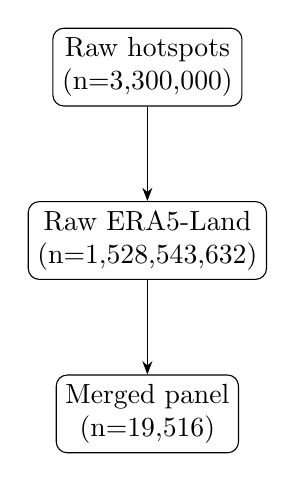
\begin{tikzpicture}[
    node distance=1.2cm,
    >=Stealth,
    every node/.style={draw, rectangle, rounded corners, align=center}
  ]
    % Nodes with actual counts
    \node (rawhot)  {Raw hotspots\\(n=3,300,000)};
    \node (raweraw) [below=of rawhot] {Raw ERA5-Land\\(n=1,528,543,632)};
    \node (panel)   [below=of raweraw] {Merged panel\\(n=19,516)};
    % Arrows
    \draw[->] (rawhot) -- (raweraw);
    \draw[->] (raweraw) -- (panel);
  \end{tikzpicture}
  \label{fig:etl_flow}
\end{figure}

\end{document}
